\begin{task}{5, Analysis and visualization of results}
\paragraph{Adding recovery}
To add a recovered state we assign recovered pedestrians to the group id for recovered individuals. To make recovery work we first added the attribute \verb+recoveryRate+ to \verb+AttributesSIRG.java+. Similar to decoupling the infection rate probabilities from the time-steps we used the same expression $(1-p)^t$ as in Task 4.6, where $p$ is the probability to recover and $t$ is the delta time since the last time-step. At the end of the \verb+update(...)+ function in \verb+SIRGroupModel.java+ we check if pedestrians have recovered and then assign them to the recovered group id accordingly. Due to the simulation visualizing pedestrians according to groups, the simulation will change the colors of pedestrians for recovered individuals to blue. 

\paragraph{Test 1}
In this test we repeat the test from task 4.5.1, where we had 1000 static pedestrians in an large area. Out of those 1000 pedestrians 990 are susceptible and 10 are infected. Unlike in task 4.5 pedestrians are now able to recover. We used the following parameters for the experiment:
\begin{verbatim}
"infectionsAtStart" : 10,
"infectionRate" : 0.05,
"infectionMaxDistance" : 10.0,
"recoveryRate" : 0.1
"infectionRateWhenAdded" : 0.0
\end{verbatim}
Once 50\% of the pedestrians had been infected we will also observe recovered pedestrians as shown below in Figure \ref{fig:task5t1other}(a). We can observe that a majority of the pedestrian have already become recovered in this case. Plotting the overall amount of susceptible, infected and recovered pedestrians over time we receive graphs seen in Figure \ref{fig:task5t1other}(b), which furthermore confirms our initial observations. Here we see the rapid decline in susceptible pedestrians as they become infected. As for the infected pedestrians we see an increase at the start, but due to the higher recovery rate the amount of infected pedestrians quickly declines to zero. Consequently we see a steady rise in recovered pedestrians.

\begin{figure}[H]
\centering
\subfigure[Infection rate 0.01 with recovery rate 0.1 at second 37]{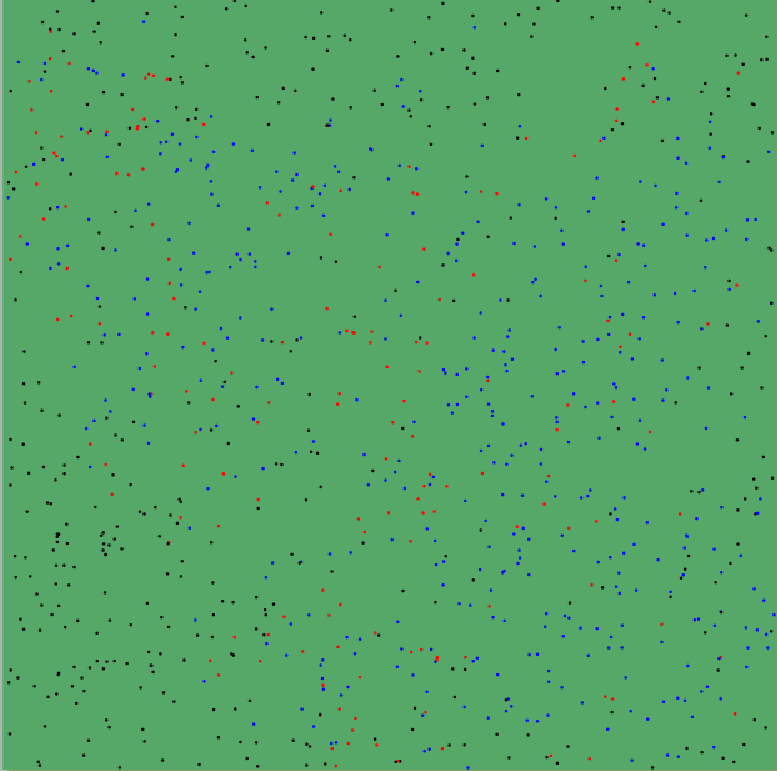
\includegraphics[width=0.4\textwidth]{report-template/images/001_recovery_37_0.png}}
\subfigure[Infection rate 0.01 with recovery rate 0.1 SIR curves]{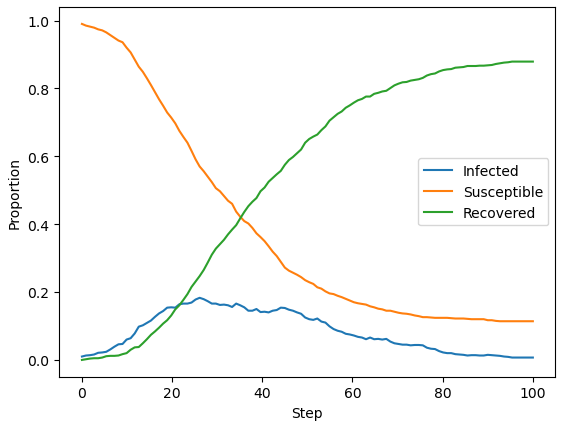
\includegraphics[width=0.45\textwidth]{report-template/images/recoverplot.png}}
\caption{Test 1 observations}
\label{fig:task5t1other}
\end{figure}

\paragraph{Test 2}
In this section we perform further tests based on the scenario given in the previous section "Test 1". In this test we experiment with different infection rates and recovery rates, which are captioned below the figures \ref{fig:task5t1}(a)-(h) as $(infectionRate, recoveryRate)$. The graphs show on the x-axis the time-step and on the y-axis the percentage of pedestrians in each group. Additionally we added a ratio $r=\frac{infectionRate}{recoveryRate}$. The graphs are sorted in ascending order of the ratio $r$.

We can generally observer that with increasing infection rate, the amount of infected increases exponentially faster, which also shows in the faster decrease in susceptible pedestrians. Similarly we observe that faster recovery rates lead to an exponential increase in recovered pedestrian which saturates eventually. Notably in Figure \ref{fig:task5t1prevention}(c) we observe that with significantly higher recovery rate the infection is unable to spread to all susceptible individuals. Hence the recovery curve is much steeper and saturates much earlier on. In \ref{fig:task5t1prevention}(a) we can see that having the recovery rate be only slightly higher does not produce the same effect. In \ref{fig:task5t1prevention}(b) we can see that having the recovery rate be 6 times the infection rate with our infection radius leaves only few pedestrians uninfected and is therefore close to the threshold.

% In the figure \ref{fig:task5t0} we see a snapshot of the simulation with infection rate $0.0003$ and recovery rate $0.0002$ at second 60.
%\begin{figure}[H]
%\centering
%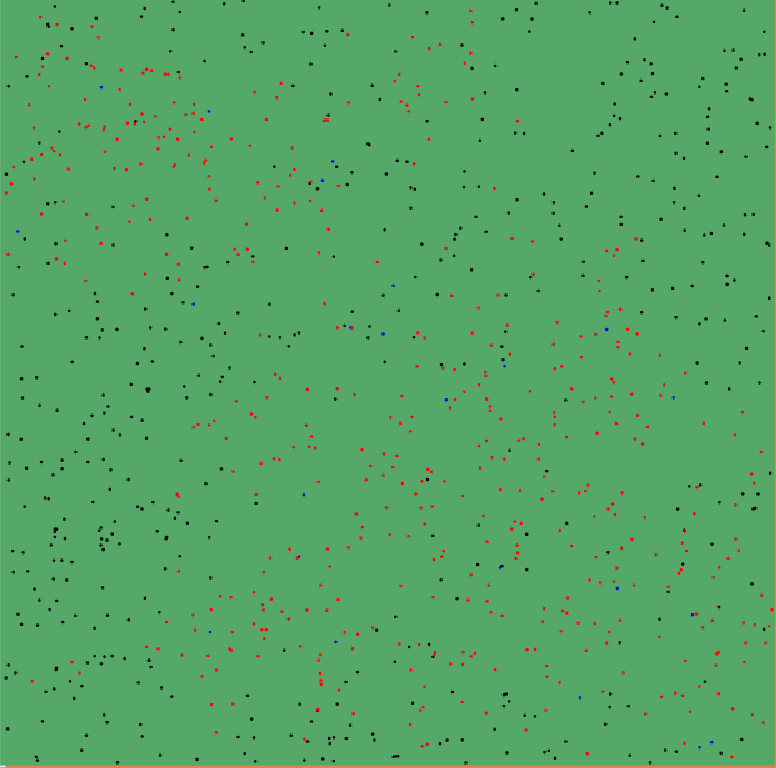
\includegraphics[width=0.4\textwidth]{report-template/images/00030002sec60.png}
%\caption{Test 2 simulation at second 60 with parameters (0.0003, 0.0002)}
%\label{fig:task5t0}
%\end{figure}

\begin{figure}[H]
\centering
\subfigure[(0.01, 0.01), r=1]{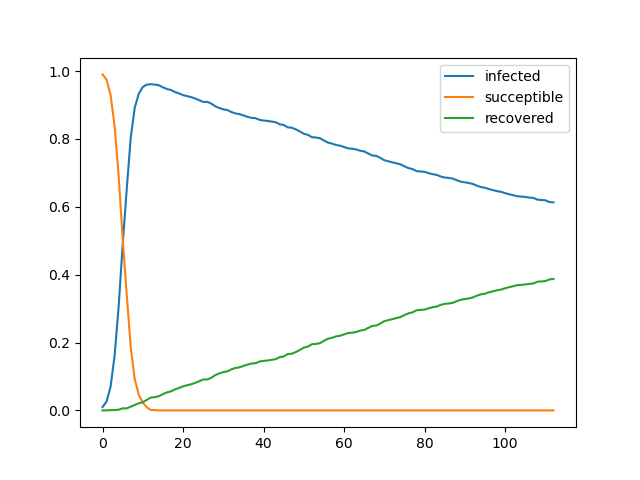
\includegraphics[width=0.35\textwidth]{report-template/images/005;0005.png}}
\subfigure[(0.07, 0.05), r=1.4]{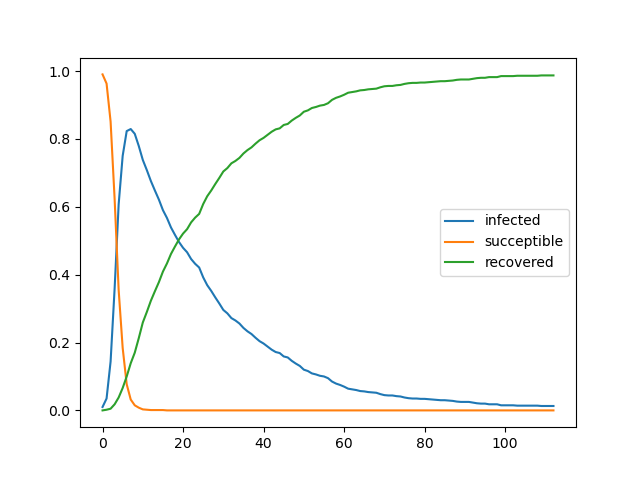
\includegraphics[width=0.35\textwidth]{report-template/images/007;005.png}}
\subfigure[(0.001, 0.0007), r=1.429]{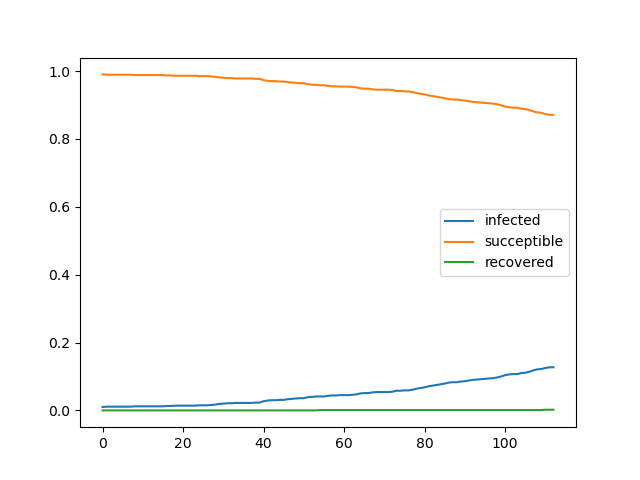
\includegraphics[width=0.35\textwidth]{report-template/images/0001;00007.png}}
\subfigure[(0.01, 0.007), r=1.429]{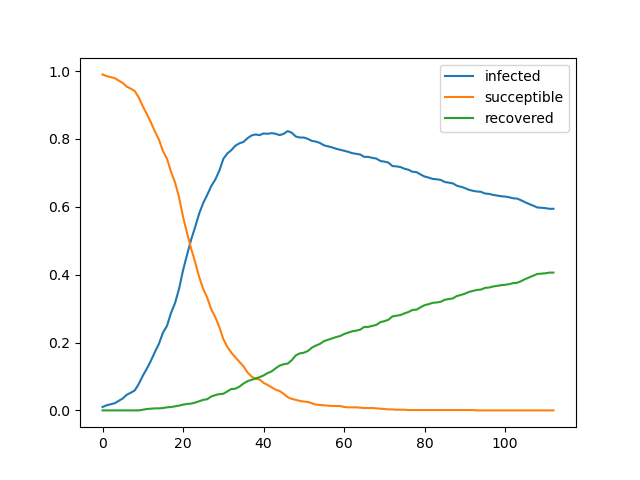
\includegraphics[width=0.35\textwidth]{report-template/images/001;0007.png}}
\subfigure[(0.003, 0.002), r=1.5]{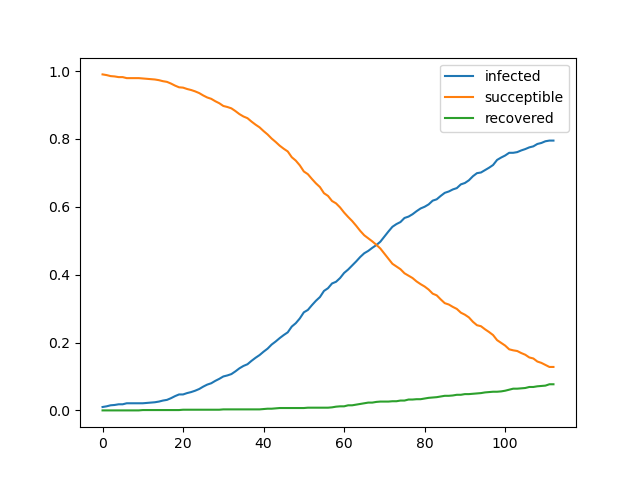
\includegraphics[width=0.35\textwidth]{report-template/images/0003;0002.png}}
\subfigure[(0.05, 0.005), r=10]{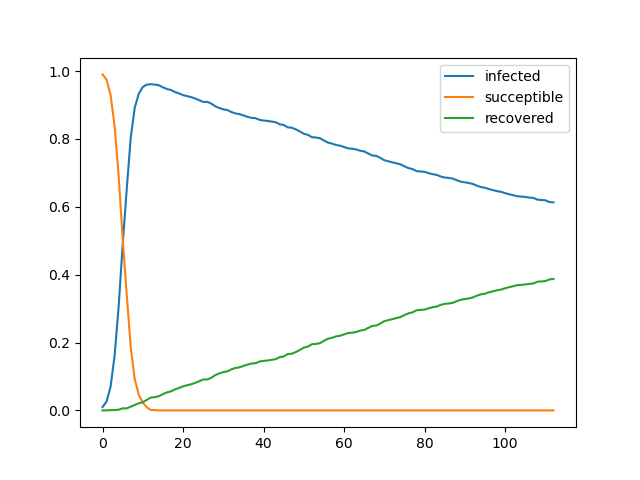
\includegraphics[width=0.35\textwidth]{report-template/images/005;0005.png}}
\caption{Test 2 observations}
\label{fig:task5t1}
\end{figure}

\begin{figure}[H]
\centering
\subfigure[(0.005, 0.05), r=0.1]{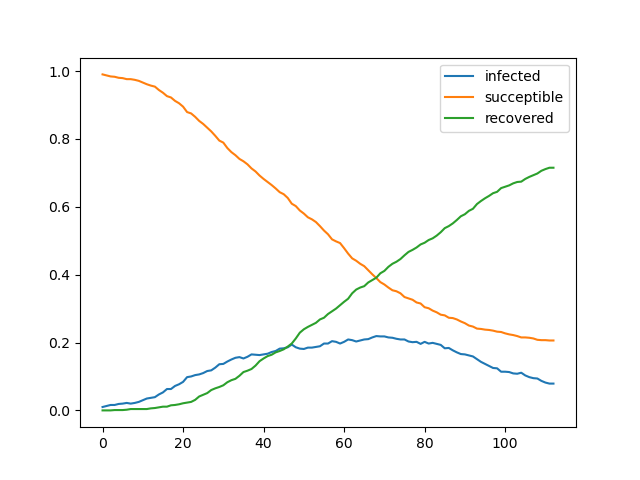
\includegraphics[width=0.35\textwidth]{report-template/images/0005;005.png}}
\subfigure[(0.01, 0.06), r=0.166]{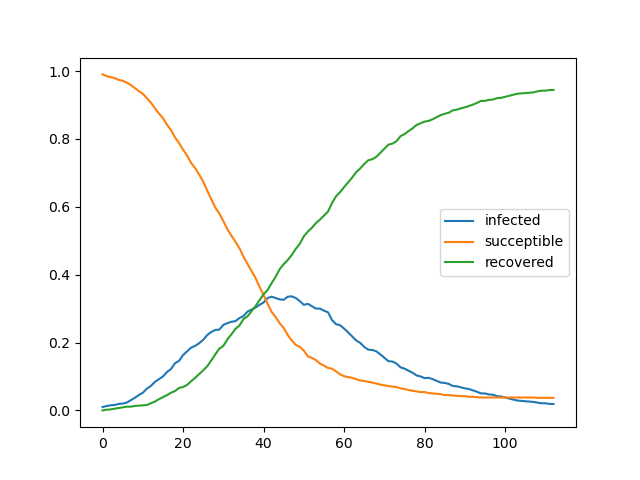
\includegraphics[width=0.35\textwidth]{report-template/images/10;60;166.png}}
\subfigure[(0.01, 0.015), r=0.66]{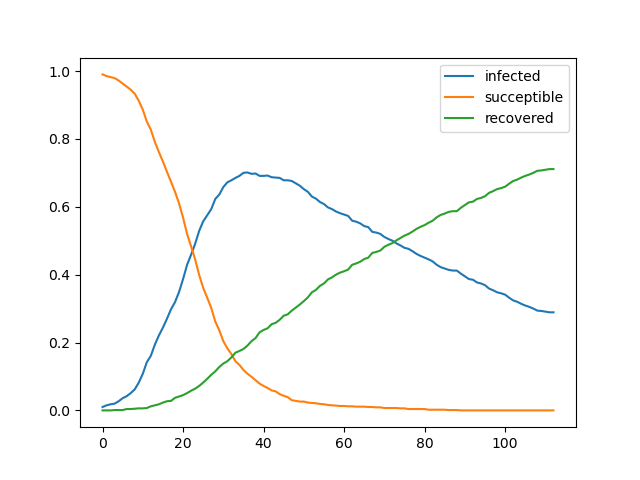
\includegraphics[width=0.35\textwidth]{report-template/images/10;15;666.png}}
\caption{Test 2 preventing infection of all pedestrians}
\label{fig:task5t1prevention}
\end{figure}

Table of parameters\ref{task5table}: Here again an overview of the parameters and their ratios used for the graphs in \ref{fig:task5t1} and \ref{fig:task5t1prevention}.
\begin{center}
\begin{tabular}{ |c|c|c|c| } 
 \hline
Figure & Infection Rate (IR) & Recovery Rate (RR) & IR/RR-Ratio\\
\hline
\ref{fig:task5t1}a & 0.01 & 0.01 & 1 \\
\hline
\ref{fig:task5t1}b & 0.07 & 0.05 & 1.4\\
\hline
\ref{fig:task5t1}c & 0.001 & 0.0007 & 1.429\\
\hline
\ref{fig:task5t1}d & 0.01 & 0.007 & 1.429\\
\hline
\ref{fig:task5t1}e & 0.003 & 0.002 & 1.5\\
\hline
\ref{fig:task5t1}f & 0.05 & 0.005 & 10\\
\hline
\ref{fig:task5t1prevention}a & 0.005 & 0.05 & 0.1\\
\hline
\ref{fig:task5t1prevention}b & 0.01 & 0.06 & 0.167\\
\hline
\ref{fig:task5t1prevention}c & 0.01 & 0.015 & 0.667\\
\hline
\end{tabular}
\label{task5table}
\end{center}


\paragraph{Supermarket test}
In order to test the infection model in a real-case scenario, we have designed a supermarket inspired on the ALDI SÜD at Wotanstraße 9c (Figure \ref{aldi-scen}a). This supermarket is not very big so it is one where infections are more likely to occur. The supermarket has a main door where the checkouts are placed in front. To enter the actual supermarket, you enter through the left zone of the door, where the fruit and vegetable area is located with the meat shelves in front, a place that as we will see is quite crowded. Then, one of the most prominent areas is the corridor at the end on the left, where the dairy products are, as well as pasta, eggs and other foodstuffs that are quite necessary in people's diets. This is also where a lot of people tend to accumulate (We have personally verified this).
Then, we have different aisles with less required foods such as biscuits, soft drinks and alcoholic beverages, as well as cleaning products. Behind the checkouts, the supermarket has its freezer and clothing sections.

We have modelled the scenario in such a way that we try to faithfully imitate the crowds of people we have seen during our personal experience in the supermarket. So each aisle has targets, which is where people tend to go and stand. For example, the last aisle on the left is one of the most populated ones, so it has more areas where people go interested in what's there. However, the corridor next to it contains refreshments and water, so apart from being less crowded, people don't tend to walk the whole aisle (Figure \ref{aldi-scen}b).

Finally, we also created a variety of sources, where each of them spawn different types of customers. For example, one of them models a type of customer who makes a complete purchase (meat, vegetables, pasta, drinks, cleaning products, goes to the checkout and leaves). Another models a type of customer who simply wants snacks so his path is shorter and more direct (he goes to the biscuit aisle, the snack aisle, goes to the checkout and leaves). Then we basically added variations of these two main customer types (long path and short path). One source generates pedestrians who buy food to host a party (snacks, alcoholic beverages and soft drinks) or another source generates customers who do a complete shopping, but instead of cleaning products they buy frozen food. In addition, we observed that most people do complete purchases, so this is also modelled. There will be more people of the first type of customer than of the second type.

We achieve this behaviour of the pedestrians adding a list of targets to the source and setting the targets' absorber property to false.

\begin{figure}[H] 
\centering
\subfigure[A photo of the supermarket from the checkout]{
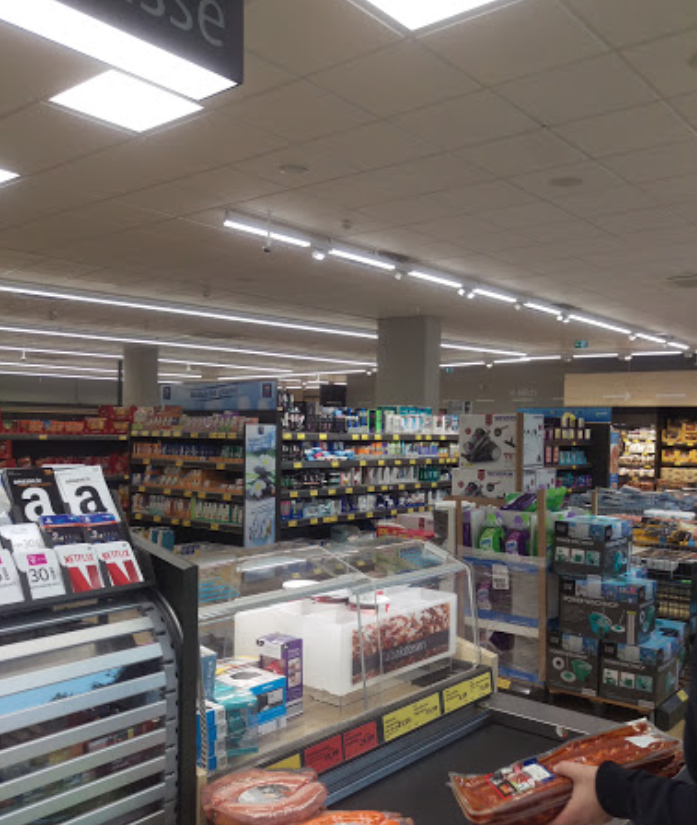
\includegraphics[scale=0.25]{report-template/images/supermarket_snapshot.png}}
\subfigure[The supermarket scenario]{
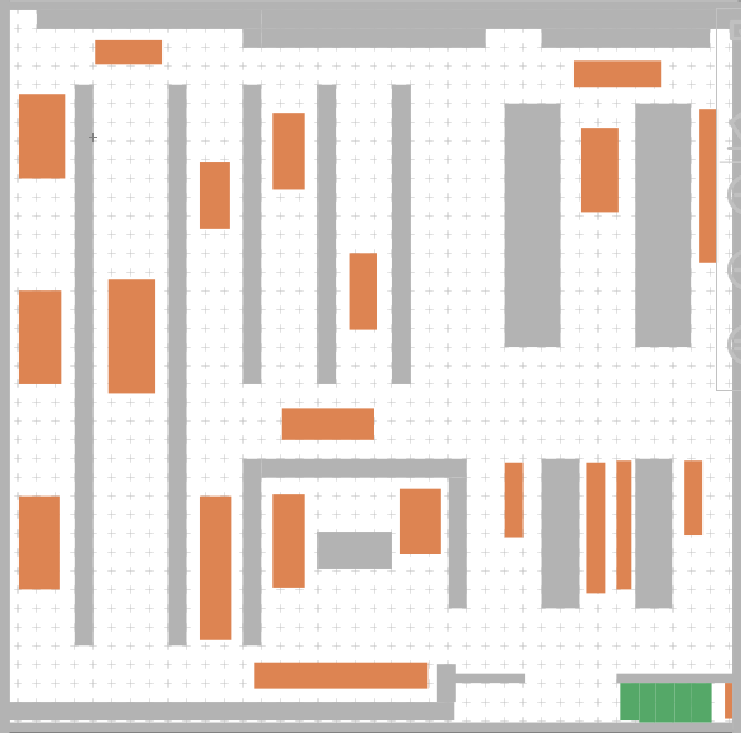
\includegraphics[scale=0.35]{report-template/images/supermarket_scen.png}}
\caption{Modelling of the ALDI SÜD}
\label{aldi-scen}
\end{figure}

After designing the scenario, we can start to test the model in it. 

We did a dual test on the scenario. First, we observed how the model behaves without social distancing, and then we test the simulation with social distancing. 

The attributes for the SIR model are same for both test:
\begin{verbatim}
"org.vadere.state.attributes.models.AttributesSIRG"
\end{verbatim}
are these
\begin{verbatim}
"infectionsAtStart" : 0,
"infectionRate" : 0.05,
"infectionMaxDistance" : 1.0,
"recoveryRate" : 0.0,
"infectionRateWhenAdded" : 0.2
\end{verbatim}


However, the attributes for \verb+org.vadere.state.attributes.models.AttributesPotentialCompactSoftshell+
are different in both cases. 

In the test without social distancing we have the following attributes:
\begin{verbatim}
"pedPotentialIntimateSpaceWidth" : 0.2,
"pedPotentialPersonalSpaceWidth" : 0.5,
"pedPotentialHeight" : 50.0,
"obstPotentialWidth" : 0.8,
"obstPotentialHeight" : 6.0,
"intimateSpaceFactor" : 1.2,
"personalSpacePower" : 1,
"intimateSpacePower" : 1
\end{verbatim}

We decrease the \verb+pedPotentialIntimateSpaceWidth+ space in order to be able decrease the \textbf{pedPotentialPersonalSpaceWidth} because our scenario is quite small and we need the personal space to be smaller than the infection radius (precisely half).

In the test with social distancing \verb+pedPotentialPersonalSpaceWidth+ is increased to 2.0 to double the infection radius so the difference is substantial enough to distinguish from noise.

\begin{figure}[H]
\centering
\subfigure[Difference between distancing test]{
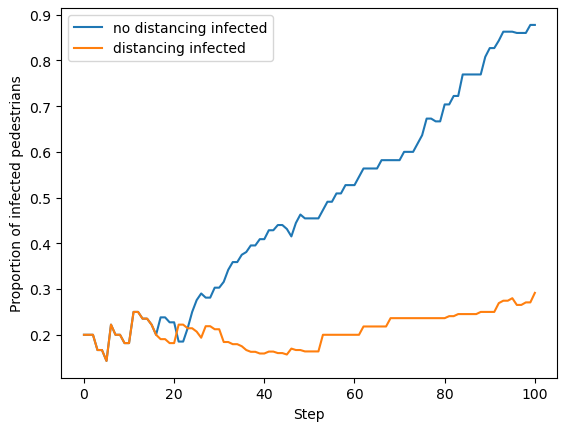
\includegraphics[width=0.45\textwidth]{report-template/images/socialvsno.png}}
\subfigure[Simulation with social distancing]{
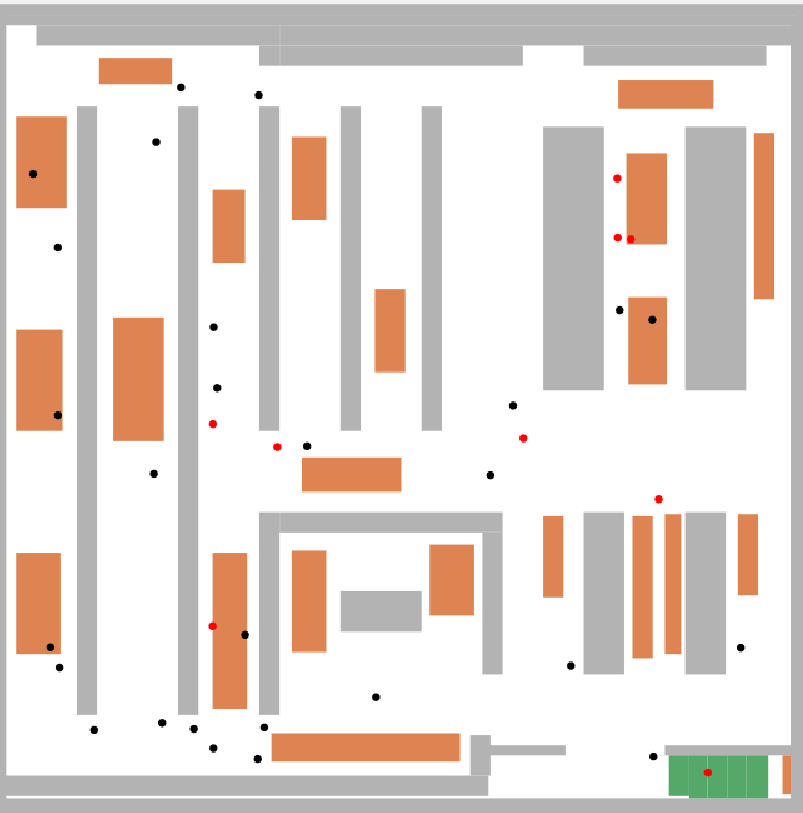
\includegraphics[scale=0.40]{report-template/images/social_distancing.png}}
\caption{Supermarket test with and without social distancing}
\label{socialvsnosocial}
\end{figure}

As we can observe in Figure \ref{socialvsnosocial}a, it is very clear that the distancing is helping to prevent the infection from spreading. In the test without social distancing, the 90\% of the pedestrians get infected in the end of the simulation, whereas with social distancing, the proportion of infected pedestrians remains almost constant, not surpassing the 30\% of infected people.

In addition, we have made a study about the most dangerous zones. Given the intersections of the paths that pedestrians follow, i.e. the areas that will have the highest density as more paths pass through them; we can detect which are the zones with more probability to spread the infection. According to our model's paths based on our real experience in the supermarket, the main ones are these 2 zones:
\begin{itemize}
    \item \textbf{Vegetable, fruit and meat zone}: Many paths coincide in the vegetable, fruit and meat zone, mainly because is the entrance and the food in that zone is very demanded (that's why there are 3 targets very close).
    \item \textbf{Supermarket check-outs}: Obviously the other zone where all the paths converge are the supermarket check-outs, being a zone that can reach high densities of people. However, in the model is less dangerous that in the real world, as it is not implemented in the scenario that pedestrians have to wait their turn. So they pass by, being less populated because each pedestrian arrives in different steps at the check-out depending on their path.
    
\end{itemize}
Also, the last corridor on the left is a very crowded place where many paths converge, as we commented in the designing of the scenario, but being a little less dangerous as pedestrians go in the same direction.

\begin{figure}[H]
\centering
\subfigure[People entering the danger zone at time $t$]{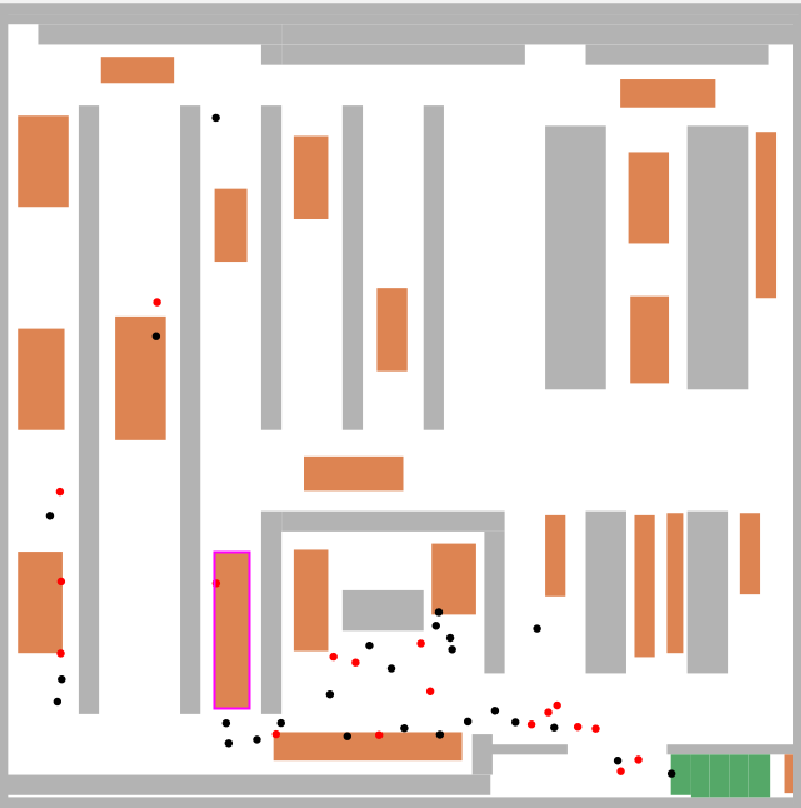
\includegraphics[width=0.4\textwidth]{report-template/images/supermarket_snap2.png}}
\subfigure[Simulation at $t+2$]{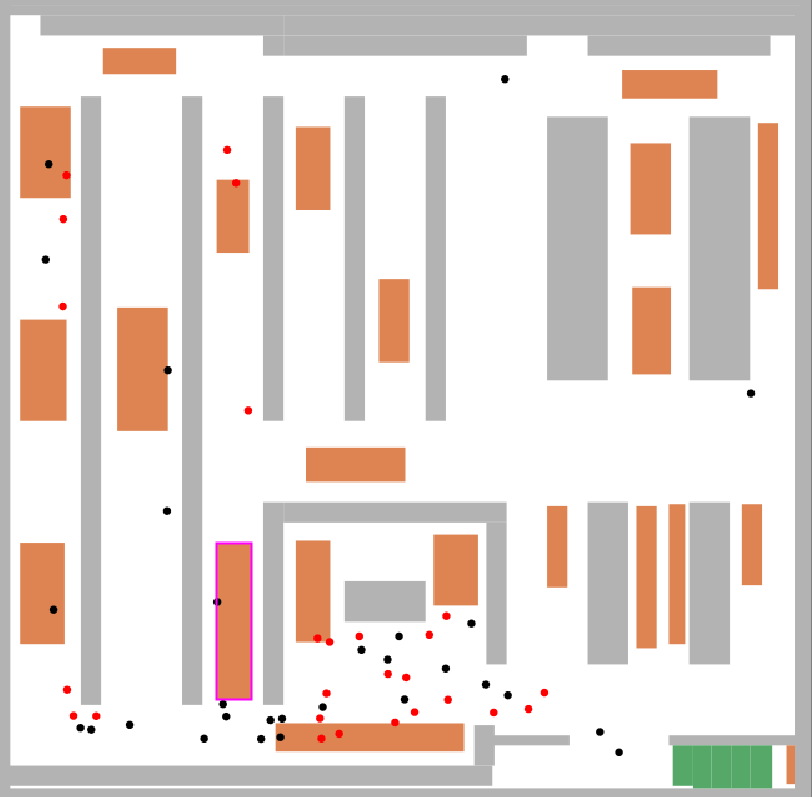
\includegraphics[width=0.4\textwidth]{report-template/images/supermarket_snap1.png}}
\caption{Vegetable, fruit and meat zone}
\label{infectvege}
\end{figure}


An example of a danger zone can be viewed in Figure \ref{infectvege}, where we can observe one of the highest density of people, and thus, a potential infection point. 

Moreover, in Figure \ref{socialvsnosocial}, the increment of infected people is almost linear without social distancing. On the other hand, with social distancing, in spite of being mainly constant, we can observe that the highest infection rates are achieved in the beginning and in the end, coinciding with the entrance to the vegetable, fruit and meat area, and the supermarket checkouts respectively.

In short, although social distancing keeps infection under control at less than 30\%, this is still a high number in the case of a real scenario. We believe that the best way to reduce the number of infected without restricting too much the number of customers that can enter the supermarket, would be to change mainly the organization of the danger zones. Therefore, if you know that meat, fruit and vegetables are very demanded, increasing the distance between each other would be helpful. Also, it would be good that the most demanded food is not in front of the door of the supermarket, as this ALDI horribly does, forcing the paths of all possible types of customers to coincide in this already crowded area. On the other hand, check-outs are more difficult to manage as every customer's path need to pass through there. It would be a suitable option, if possible, to provide two or more check-out areas with their respective doors to the outside, so as to reduce the density in each of them.

\paragraph{Bonus tests: TUM Main Campus exit}
For the bonus tests we have created a new scenario imitating another real case that we have experienced: Leaving TUM's main campus when classes are over.

Simplifying the actual architecture of the university exit, the scenario consists of two corridors, facing each other, with classes in each. The class exits are modelled as sources, which are placed opposite each other along the corridor. Looking at the number of people in a TUM class we have assumed that each class contains 30 people.

The aim of the simulation is to test how the infection spreads in a common and chaotic situation such as a school exit, where all pedestrians have a very similar path. We have modelled the two doors through which students must pass to reach the actual exit, which is more extensive, as two targets. 

This way, pedestrians are forced to pass through but it also allows us to have control over which gate pedestrians will use. Therefore, to better simulate a real situation, we have forced two groups of pedestrians, each of them belonging to a classroom, to go through the opposite door to the one closest to them, as sometimes happens in reality, where there are people who go through the door that a priori is the least intuitive.

\begin{figure}[H]
\centering
\subfigure[Entrance/exit TUM Main campus]{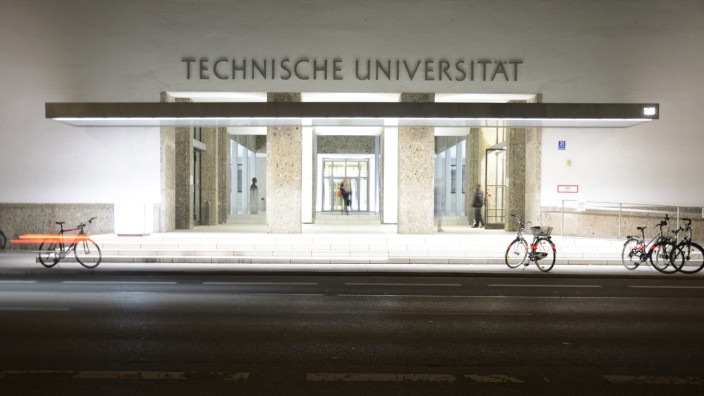
\includegraphics[width=0.4\textwidth]{report-template/images/tum_real.jpeg}}
\subfigure[Scenario]{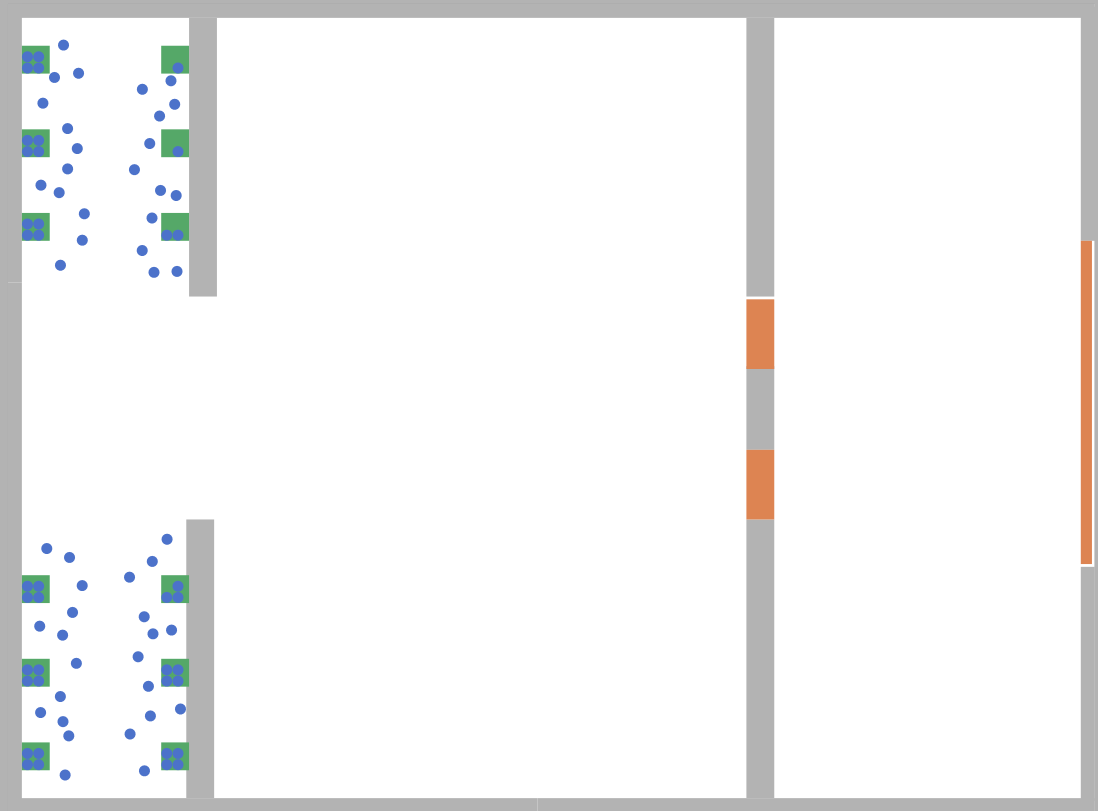
\includegraphics[width=0.4\textwidth]{report-template/images/tum_exit.png}}
\caption{TUM Main campus exit modelling}
\label{tumscen}
\end{figure}

We have added 10 infected pedestrians to the northern group. In this way, we will be able to observe how the infection spreads and if it reaches people coming out of the southern corridor.

First, we have done a test without social distancing. As we can observe that, cause of not having social distancing, almost all northern pedestrians get infected before leaving the corridor, as they accumulate on the wall, sticking closely together (Figure \ref{tumnodist}). Also, we can see how the pedestrians that belonged to the southern group that pass through the northern gate (the black dots that are transferred to the other group), become infected. Then, the infected group that goes through the southern gate infects most of the healthy ones, reaching 80\%, as shown in Figure \ref{tumnodist}c.
\begin{figure}[H]
\centering
\subfigure[Simulation middle]{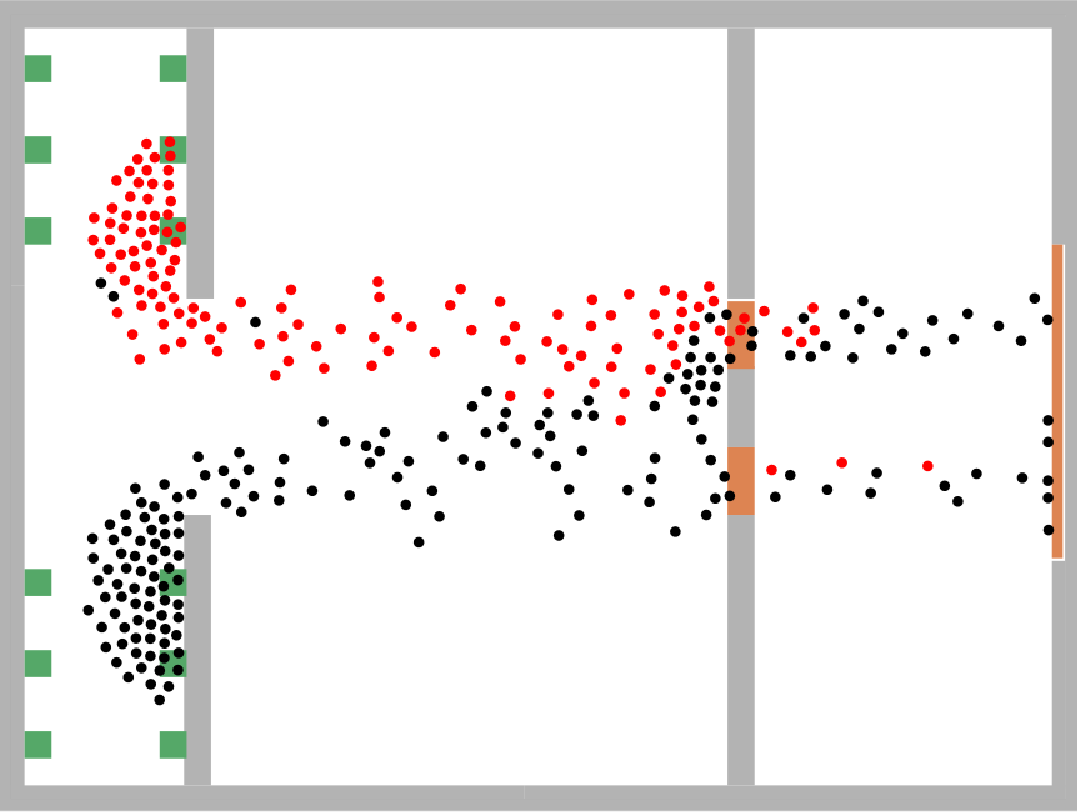
\includegraphics[width=0.4\textwidth]{report-template/images/nosocial1.png}}
\subfigure[Simulation finish]{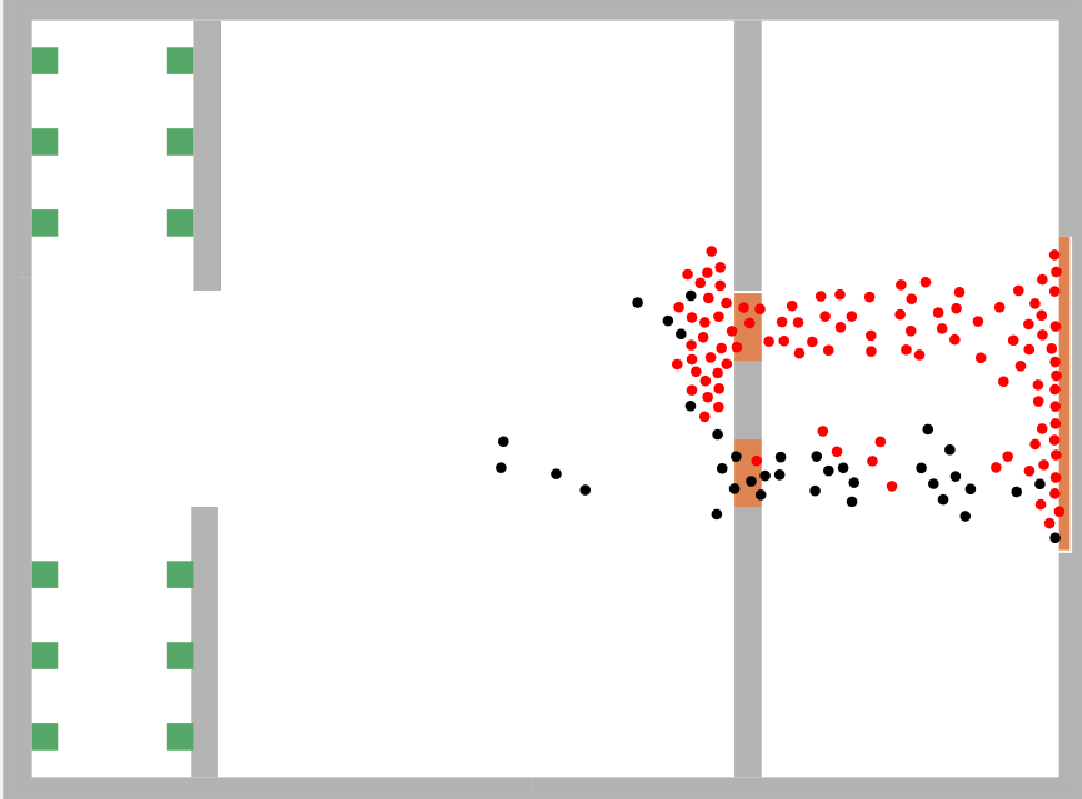
\includegraphics[width=0.4\textwidth]{report-template/images/nosocial2.png}}
\subfigure[Percentage of infected over time]{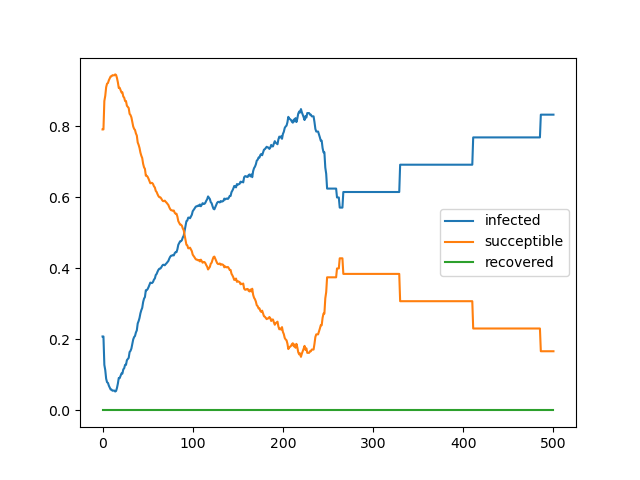
\includegraphics[width=0.45\textwidth]{report-template/images/withoutdistancigplot.png}}
\caption{Simulation without social distancing}
\label{tumnodist}
\end{figure}
Moreover, in the plot we can observe how the infection grows very fast at the start, when all pedestrians start to accumulate on the wall (until the middle of the graph). Obviously, there a no recovered pedestrians, not making sense in this real case scenario. After the middle of the graph, we can observe how the amount of people is reduced in a kind of pattern, being this a sign that the pedestrians are exiting the door, i.e. reaching the final target and disappearing in a ordered pattern.

In the test with social distancing, we can see that this time the pedestrians do not all pile up together when leaving the classroom, allowing those already infected to move on without infecting the entire corridor population (Figure \ref{tumdist}a). However, as soon as they reach the area of the two doors, it is more difficult to separate, and added to the fact that groups of infected people enter the south door, where most of the healthy people are, the proportion of infected people increases (Figure \ref{tumdist}b). Finally we can observe this behaviour looking at Figure \ref{tumdist}c, where the slope of the graph is a little gentler at the beginning, but steepens when most of the pedestrians reach the danger zone of the two gates, until it finally reduces the population when exiting. We can also observe that with social distancing pedestrians arrive earlier to the exit, due to a less bottleneck in the two corridors.
\begin{figure}[H]
\centering
\subfigure[Simulation start]{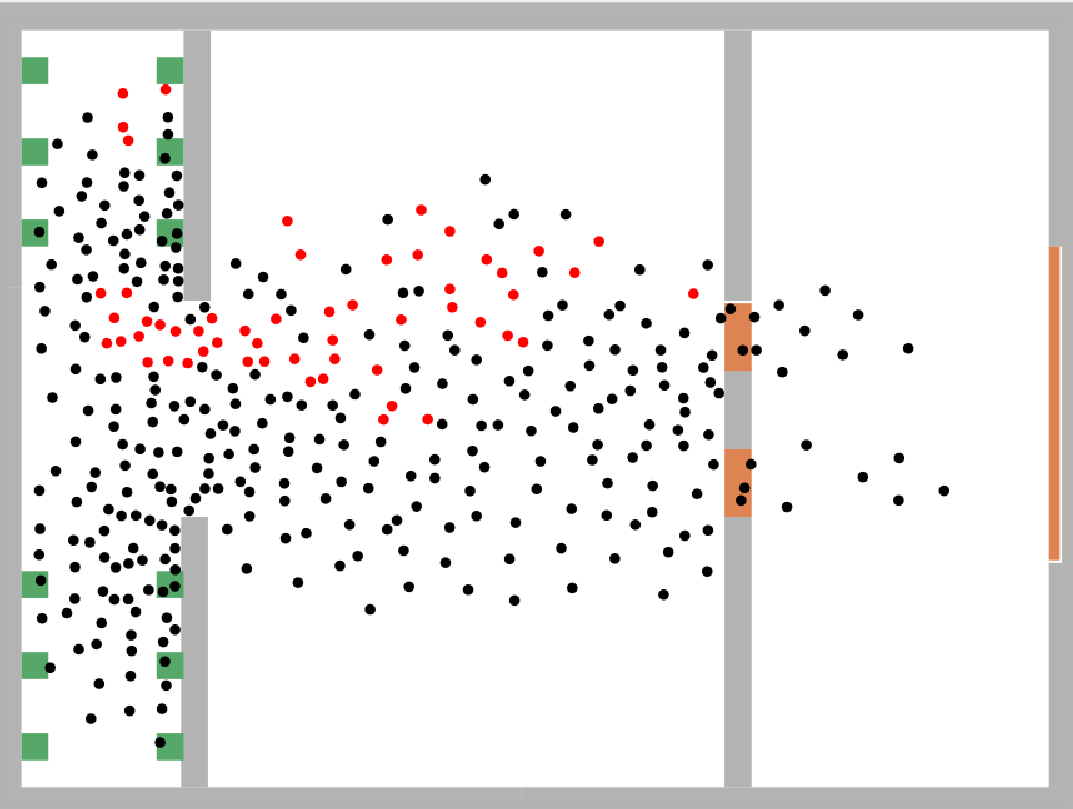
\includegraphics[width=0.4\textwidth]{report-template/images/distancing1.png}}
\subfigure[Simulation middle]{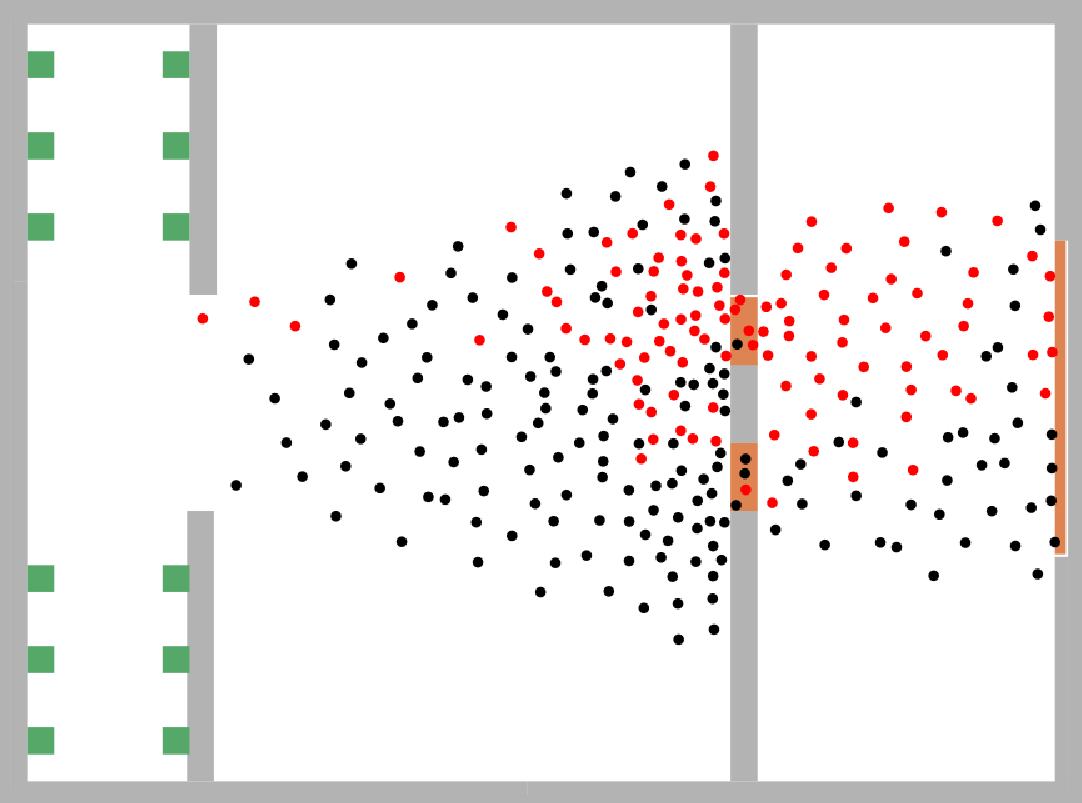
\includegraphics[width=0.4\textwidth]{report-template/images/distancing2.png}}
\subfigure[Percentage of infected over time]{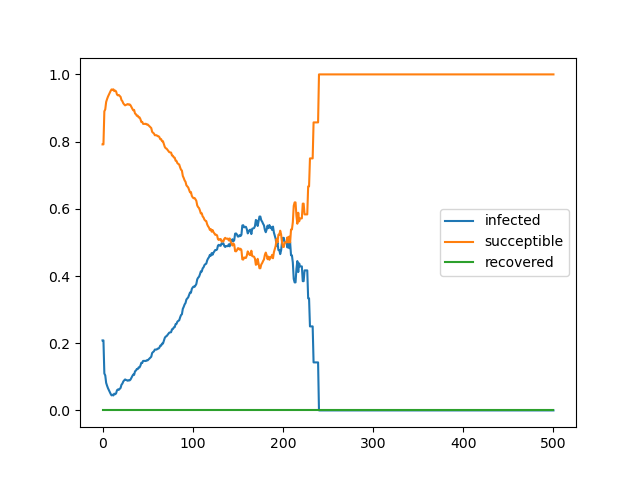
\includegraphics[width=0.45\textwidth]{report-template/images/plotdistancing.png}}
\caption{Simulation with social distancing}
\label{tumdist}
\end{figure}

Finally, comparing both experiments' plots, it can be seen that social distancing reduces the extent of infection to 60\% in contrast with 80\% obtained without social distancing. However, in both cases the infection reaches a high proportion of the population, showing us that this scenario in a real-life situation is dangerous and should be treated with caution. Assuming that the architecture of the building cannot be changed, we think that the best way to leave the Main campus of Tum in an infection situation is by individually organizing the classes to leave at a certain time each, avoiding contact with the rest of the classes at the exit and in the corridors.
\end{task}